\section*{Problem 1}

\begin{enumerate}
  \item Stable Node: \textbf{Asymptotically Stable}
  \item Unstable node: \textbf{Unstable}
  \item Stable Focus: \textbf{Asymptotically Stable}
  \item Unstable Focus: \textbf{Unstable}
  \item Center: \textbf{ Stable}
\end{enumerate}

\subsection*{Part 1}
A stable node is asymptotically stable since it all trajectories will trend to the origin (aka node) as \textbf{t} goes to $\infty$. While stability states that given an initial condition the trajectory of the solution will be bounded, asymptotic stability states that the trjectory will trend towards zero as time goes to $\infty$

\begin{center}
  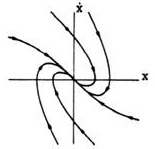
\includegraphics{stable_node}
\end{center}

\subsection*{Part 2}
By definition, an unstable node, is unstable. However this can be seen via it's phase portrait where any trajectory starting from the initial condition deviates away from the origin (not asymptotically stable) and further more does not stay in a bounded neighborhood (no stable). Since neither of these traits are present, the system is \textbf{unstable}.

\begin{center}
  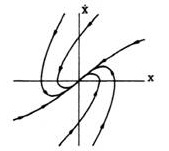
\includegraphics{unstable_node}
\end{center}

\subsection*{Part 3}
A stable focus is asymptotically stable since it all trajectories will trend to the origin. This assertion is clear from it Phase Portrait, that any trajectory started from any initial condition will spiral into the origin. This agrees with the definition of \textbf{asymptotic stability} all trjectories will trend towards zero (the origin) as time goes to $\infty$

\begin{center}
  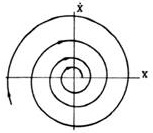
\includegraphics{stable_focus}
\end{center}

\subsection*{Part 4}
By definition, an unstable focus is unstable. However, it is clear from the phase portrait that all trajecories from an initial condition will invariably trend away from the origin. Since the trajectories do not converge to the origin, and since the tracjectories do not stay bounded in some neighborhood they are unstable

\begin{center}
  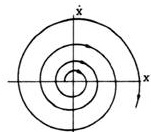
\includegraphics{unstable_focus}
\end{center}

\subsection*{Part 5}
A center is stable since it stays we can find some neighborhood about the origin in which the trajectory of the center is orbiting. However, as is clear from the phase portrait, since the center does not converge to the origin but oscillates around it, it cannot be asymptotically stable since the trajectory of the center does not converge to the origin, but merely orbits it.

\begin{center}
  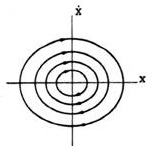
\includegraphics{center}
\end{center}
